\documentclass[a4paper]{article}

%% Language and font encodings
\usepackage[english]{babel}
\usepackage[utf8]{inputenc}
\usepackage[T1]{fontenc}

%% Sets page size and margins
\usepackage[a4paper,top=3cm,bottom=2cm,left=3cm,right=3cm,marginparwidth=1.75cm]{geometry}

%% Useful packages
\usepackage{amsmath}
\usepackage{graphicx}
\usepackage[colorinlistoftodos]{todonotes}
\usepackage[colorlinks=true, allcolors=blue]{hyperref}
\usepackage[numbers]{natbib}
\usepackage{dblfloatfix}
\usepackage{subcaption}
\usepackage{floatrow}
\usepackage{multirow}
\usepackage{authblk}


\newfloatcommand{capbtabbox}{table}[][\FBwidth]
\usepackage{calrsfs}
\DeclareMathAlphabet{\pazocal}{OMS}{zplm}{m}{n}
\newcommand{\Sc}{\mathcal{S}}
\newcommand{\Sa}{\pazocal{S}}


\title{Comparison of solution approaches for the Set Cover Problem}
\author{Dominik Ramsauer, Matrikelnummer: 1737690}
\affil{Lehrstuhl für Informationswissenschaft, Universität Regensburg}

\begin{document}
\maketitle

\begin{abstract}
The Set Cover Problem is a research issue in computer science with a lot of applications e.g. in machine learning, data mining and information retrieval. It is about selecting as few sets as possible from a collection that cover some universe. The aim of this project is to compare two approaches - a deterministic one and a statistical - and to rate them by concerns of coverage rate, solution size and computation time. 
\end{abstract}

\section{Introduction}

The \textbf{Set Cover Problem} is a research issue in computer science, combinatorics and computational complexity theory which finds applications in machine learning, data mining/information retrieval\cite{saha2009maximum}, wireless sensor networks\cite{Zorbas2010} and web host analysis\cite{chierichetti2010max} as also in learning theory\cite{kearns1994introduction} and operation research\cite{grossman1997computational}. In simple terms, the issue of the problem is about selecting as few sets as possible from a collection that cover some universe\cite{Cormode,Feige1998}. The Set Cover problem is known to be NP-hard and finding an optimal solution is NP-complete \cite{Indyk}. Richard M. Karp stated in 1972 21 NP-complete problems\cite{Karp2010}, where the Set Cover Problem is also mentioned. This means that there is no algorithm existing, which finds an optimal solution in polynomial time. 

Therefore, the problem needs to be approximated properly. Even though algorithms based on a greedy heuristic are the most used to solve it, there are a bunch of other approaches discussing the Set Cover problem. For this project we want to consider two kinds of algorithms in particular: deterministic algorithms on one hand and statistical algorithms on the other hand. One for each of those two attempts is to be presented in this work - a kind of tuned greedy algorithm for the deterministic attempt as presented in \cite{Cormode} and the so called simulated-annealing algorithm \cite{Jacobs1995,balas1980set,Kirkpatrick1983, vcerny1985thermodynamical}, which was inspired by a technique in metallurgy. The aim of this project is two compare these approaches and to rate them by concerns of coverage rate, solution size and computation time.

\section{Technical Definitions and Algorithms}

\subsection{The Set Cover Problem}
For this project we concentrate on the standard Set Cover problem, meaning that all sets unweighted \cite{Alon2003}. We have given a collection $\Sc = \{S_1,S_2,..., S_m\}$ of size $|\Sc| = m$, our sets-universe, containing a bunch of $m$ text sets and a universe $X = \{x_1, x_2, ..., x_n\}$ of $n$ elements, our words-universe. The aim is to get a sub-collection of $\Sc$ containing as few sets as possible that covers our words-universe $X$.

The most used algorithm for approximating the Set Cover problem is based on a greedy heuristic\cite{Cormode,Feo1995,balas1980set, johnson1974approximation}. This algorithm adds sets from the collection to the solution-collection measuring the size of the sets. The intention behind this procedure is, that large sets lead potentially to a high coverage. Therefore, we define a set $\Sigma$ containing the indices of the sets that are added to our solution, and a set $C$ containing the different elements that have been covered so far. A snippet of pseudo-code is shown on the next page.
\pagebreak

\begin{tabbing}
\textbf{Procedure:}\cite{Cormode} \\
\textit{Initialization.} $\Sigma = \emptyset$, $C = \emptyset$ \\
\textit{Loop.} \= while $C$ != $X$: \\
\>1. Choose a set with $max(|S_i \backslash C|)$; let its index be $i^*$ \\
\>2. Add $i^*$ to $\Sigma$ \\
\>3. Let $C = C \cup S_i^*$ \\
\textit{Return.} $\Sigma$
\end{tabbing}

So at each step of the greedy algorithm there has to be computed, which set in the collection has the most elements that have not already been covered. In more mathematical terms: the set $|Si \backslash C|$ after subtracting all already covered elements, that has the maximum length. This procedure requires many iterations through the data set, so that it has to be read very often, or some support technique has to be implemented such as an inverted index\cite{Cormode}. Another point that has to be mentioned is, that a kind of threshold has to be implemented when the greedy procedure may stop, especially when the words-universe $X$ is not known in advance. If it is known, the greedy heuristic can be implemented in that way, that it checks at every step if all words are covered and stops at this point\cite{balas1980set, Jacobs1995}. 

The standard greedy heuristic does not accomplish to find the optimal solution in most cases, meaning that there are often shorter solutions. The approaches presented in the next sections are extensions of the greedy heuristic and had been chosen to improve it by concerns of speed and accuracy. 


\subsection{Disk-Friendly Greedy}
As the name indicates, this algorithm published by \citeauthor*{Cormode} is based on the greedy algorithm presented before. As the greedy algorithm does need many random accesses on disk, the greedy algorithm performs badly on disk resident data, especially if data is very large\cite{Cormode}. To scale the greedy procedure to large data sets they introduce a new algorithm suited for these modern claims.

The idea behind their disk-friendly greedy (DFG) is to build sub-collections of the given sets-universe by the size of the sets. They introduce a parameter $p > 1$, which will control the set-size in the sub-collections and therefore acts as a running time and approximation factor. 

Each set $S_i$ will be attached to sub-collection $\Sa^{(k)}$ if:
%\[ 
\begin{equation}
    p^k \leq |S_i| < p^{k+1}
\end{equation}
%\]
The sub-collection $\Sa^{(K)}$, with $K$ being the highest value of all $k$ where the $\Sa^{(k)}$ is not empty, is therefore the sub-collection with the biggest-sized sets. Table \ref{table:example-set} shows an example of sets from \citeauthor{Cormode} with Table \ref{table:example-sub-collections} showing how these sets are categorized at initialization by the size rule (1) presented before with $p = 2$. 

Beginning with the sub-collection $\Sa^{(K)}$ containing the largest sets, the algorithm selects a set $S_i$ in the sub-collection, and removes all elements from the set which are already covered in $C$. If the set-size is still $\geq p^k$, the algorithm adds the set index $i$ to our solution $\Sigma$ and adds the (remaining) elements to our already-covered-list $C$; If set size is now below $p^k$, the updated set will be appended to the sub-collection $\Sa^{(k')}$, where the set-size fulfills rule (1). This procedure is repeated for each set in $\Sa^{(k)}$ for each $k$ in descending order until there are only sets containing only one element. Then the algorithm simply checks if the element in the set is not already covered and updates $\Sigma$ and $C$ if so. 

      
\begin{figure}[!b]
    \textbf{Sets and sub-collection example in \citeauthor{Cormode}\cite{Cormode} }\par\medskip
    \begin{floatrow}
    \capbtabbox{
        \begin{tabular}{r|l}
            1 & ABCDE \\
            2 & ABDFG \\
            3 & AFG \\
            4 & BCG \\
            5 & GH \\
        \end{tabular}
        \begin{tabular}{r|l}
            6 & EH \\
            7 & CI \\
            8 & A \\
            9 & E \\
            10 & I
        \end{tabular}
    }{
      \caption{Sets with words universe = \{A,B,C,D,E,F,G,H,I\}}
      \label{table:example-set}

    }
    \capbtabbox{%
        \begin{tabular}{r c l}
            $\Sa^{(k)}$ & Set-Size & Set (\#)\\ \hline 
            $\Sa^{(2)}$ & 4-7 & ABCDE(1),  ABDFG(2) \\
            $\Sa^{(1)}$ & 2-3 & AFG(3), BCG(4), \\
            & & GH(5), EH(6), CI(7) \\
            $\Sa^{(0)}$ & 1 & A(8), E(9), I(10) \\
        \end{tabular}
        
    }{%
      \caption{Sub-collections at initialization of DFG}
      \label{table:example-sub-collections}
    }
    \end{floatrow}
\end{figure}

\pagebreak

\begin{tabbing}
\textbf{Disk-Friendly Greedy (DFG):}\cite{Cormode} \\
\textit{Initialization.} $\Sigma = \emptyset$, $C = \emptyset$, choose a value for $p$, build sub-collections $\Sa$ with rule (1) \\
\textit{Loop.}  \= while $k = K \xrightarrow{} 1$: \\
                \> \textit{Loop.}   \= foreach $S_i$ in $\Sa^{(k)}$: \\
                \>                  \>* \textit{If} \= $|S_i \backslash C| \geq p^k$: \\
                \>                  \>              \> 1. Add $i$ to $\Sigma$ \\
                \>                  \>              \> 2. Update $C$ \\
                \>                  \>* \textit{Els\=e}: \\
                \>                  \>              \> 1. Let $S_i \xleftarrow{} S_i \backslash C$ \\
                \>                  \>              \> 2. Add updated $S_i$ to sub-collection $\Sa^{(k')}$ with \\
                \>                  \>              \> set-size $|S_i|$ fulfilling rule (1) \\
\textit{Loop.}  \= foreach $S_i$ in $\Sa^{(0)}$: \\
                \> \textit{If}  \= $|S_i \backslash C| = 1$: \\
                \>              \>  1. Add $i$ to $\Sigma$ \\
                \>              \>  2. Update $C$ \\

\textit{Return.} $\Sigma$
\end{tabbing}

\textbf{Example.} The algorithm starts greedy-like with one of the largest sets, so it selects one of the sets in $\Sa^{(2)}$ with set-size 4-7, e.g. set $S_1 = \{A,B,C,D,E\}$. Since there are no elements covered so far ( $C = \emptyset$ ), $i=1$ is added to $\Sigma \xleftarrow{} \{1\}$, and all elements of $S_i$ are added to $C \xleftarrow{}\{A,B,C,D,E\}$. 
The algorithm continues with the next set in $\Sa^{(2)}$: $S_2 = \{A,B,D,F,G\}$. Since $C$ is not empty anymore, it checks whether set $S_2$ contains covered elements and deletes them if so. Since $S_2$ contains three covered elements ($A,B,D$), $S_2$ is updated to $S_2 \xleftarrow{} \{ F,G\}$ and is appended to a different sub-collection to fulfill the size-rule (1), in this case to $\Sa^{(1)}$. 

Continuing with the next sub-collection $\Sa^{(1)}$, the algorithm selects the first set $S_3 = \{A,F,G\}$. In considering of $C$, the only covered element in this set is A. We let $S_3 \xleftarrow{} \{F,G\}$; since this set still fulfills rule (1), we add $i=3$ to $\Sigma \xleftarrow{} \{1,3\}$, take its remaining elements and add them to \newline $C \xleftarrow{} C \cup \{F,G\};$ so until now we have covered seven of nine elements: $C = \{A,B,C,D,E,F,G\}$. Checking the other sets in $\Sa^{(1)}$, the algorithm shortens every set: $S_4 \xleftarrow{} \emptyset$, $S_5 \xleftarrow{} \{H\}$, $S_6 \xleftarrow{} \{H\}$, $S_7 \xleftarrow{} \{I\}$, $S_2 \xleftarrow{} \emptyset$. Since none of them fulfills the size rule (1) they are all appended to $\Sa^{(0)}$.

Now the algorithm takes on the second main loop: it checks every remaining set if it still contains an uncovered element after putting out all the already covered ones. In this case these are $S_5$ and $S_7$ - their indices are added to $\Sigma \xleftarrow{} \{1,3,5,7\}$ and their elements $H$ and $I$ are added to $C = \{A,B,C,D,E,F,G,H,I\}$. The algorithm now finishes and returns $\Sigma$:  $S_1$,  $S_3$, $S_5$ and $S_7$ are the sets that the algorithm has chosen. In this case it has done its job perfectly: all different elements in our example sets have been covered.




\subsection{Simulated-Annealing}
The second algorithm that is investigated in this work is based on the simulated annealing algorithm, a statistical technique to find the global optimum of a function which has become famous for solving optimization problems\cite{Jacobs1995,balas1980set,Kirkpatrick1983, vcerny1985thermodynamical}. In metallurgy, annealing is a procedure to harden metallic structures by cooling and heating materials in a controlled way so that they build larger crystals. This makes the materials free from defects an more reliable. The simulated annealing was inspired by this technique and can be applied as a metaheuristic to approximate optima. 

\citeauthor*{Jacobs1995} have published a note, in which they introduced a local-search heuristic (LSH) for the set cover problem based on simulated annealing. As the simulated annealing is a metaheuristic, an initial, feasible solution $\Sigma$ is required to start with. \citeauthor{Jacobs1995} used a greedy heuristic based on a fast approach by \citeauthor{balas1980set}. Having a feasible solution, the simulated annealing tries to find better solutions. As metric for the goodness of a solution, the solution size is chosen in this case. At initialization, three values have to be set: the temperature $T$ to start with, the temperature length $TL$, which is the number of iterations, that are done at a certain value of $T$, and the cooling factor $CF$, which reduces the temperature after each step. The values of these three parameters are not very sensitive to the quality of the solution - therefore almost the same values as in \cite{Jacobs1995} have been used, despite of the temperature length, which was reduced to only 5 iterations for saving computation time. 

\begin{table}[]
    \centering
    \begin{tabular}{0.65\textwidth}
      \hline
      Parameter & T & TL &  CF \\
      \hline 
      Value  & 1.3 & 5  & 0.9  \\
      \hline
    \end{tabular}
    \caption{Chosen parameters for \textbf{Simulated Annealing} }
    \label{tab:my_label}
\end{table}

\pagebreak

At each step of the algorithm a new solution $\Sigma'$ is searched with a search heuristic (I), which will be explained later on. After finding a new solution, we compare its length with the last solution's length. If the new solution is shorter, than it is our new best solution by now. Otherwise, we only accept the solution with a probability of ${\rm e}^{-\delta/T}$; if the probability is too low, we discard the new solution. These steps are done TL-times, until the temperature is cooled down by $CF$ $T = T \times CF$ and the loop starts again. After a chosen running time $t$, the algorithm stops optimizing.


\begin{tabbing}
\textbf{Simulated Annealing:}\cite{Jacobs1995} \\
\textit{Initialization.} \= $\Sigma = $ \textit{Feasible Solution}, $|\Sigma|$ = Length of $\Sigma$ \\
                        \> $T = $ \textit{Initial Temperature}, $TL = $ \textit{Temperature Length}, $CF = $ \textit{Cooling Factor} \\
                        \> $t = $ \textit{maximum running time .}\\
\textit{Loop.} \= while True: \\
\>\textit{Loop.} \= while $i = 1 \xrightarrow{} TL$: \\
\>\> Find a new solution $\Sigma'$ and compute its length $|\Sigma'|$ with a \textbf{Search Heuristic}  (I) \\
\>\> Let $\delta = |\Sigma'| - |\Sigma|$ \\
\>\> * \textit{If} \= $\delta <= 0$ : \\
\>\>               \> New solution is current solution: $\Sigma = \Sigma'$\\
\>\>               \> New solution is also the best solution: $\Sigma_{Best} = \Sigma'$ \\
\>\> * \textit{Els\=e}:  \\
\>\>               \> Choose a random number between $r = [0,1]$ \\
\>\>              \>* \textit{If} \= $r < {\rm e}^{-\delta/T}$: New solution is current solution: $\Sigma = \Sigma'$\\
\>\textit{Stop. If} running is higher than $t$. \\
\>Let $T = T \times CF$ \\
\textit{Return.} $\Sigma_{Best}$
\end{tabbing}

For finding a new solution at every iteration step \citeauthor*{Jacobs1995} introduced a local search heuristic. They remove randomly an amount of sets in the solution $\Sigma$ and bring then sets with a certain size to solution $\Sigma'$ again. In this work - for saving running time - the size of the sets was disregarded. The amount of removed sets $N$ is scaled by a neighbourhood-scale $p$: $N = |\Sigma| \times p $. In this approach, random sets were added to solution if they re-cover any element, that got uncovered before.

\begin{tabbing}
\textbf{Search Heuristic} based on \cite{Jacobs1995}: \\
\textit{Initialization.} \= $\Sigma' = \Sigma = $ \textit{Feasible Solution}, $U = \emptyset =$ \textit{Uncovered Elements},\\
                         \> $N = |\Sigma| \times p $ \\
\textit{Loop.} \= while $n = 0 \xrightarrow{} N: $\\
\> 1. Randomly remove a set $S_i$ from $\Sigma'$\\
\> 2. Update $U$ \\
\textit{If} $U = \emptyset$: \textit{Return.} $\Sigma'$ \\
\textit{Loop.} \= while $U != \emptyset$:\\
\>              Randomly choose a set $S_j$ from sets, that are not in solution \\
\>              \textit{Loop. }\= for each element E in $S_j$: \\
\>              \>      *\textit{If }\= $E \in U$: \\
\>              \>      \>              1. Update $U = U \setminus E$  \\
\>              \>      \>              2. Add $S_j$ to solution $\Sigma'$\\
\>              \>      *\textit{Els\=e}\= :\\
\>              \>      \>              \textit{Continue.} \\
\textit{Return.} $\Sigma'$
\end{tabbing}


\section{Experiments and Results}

\subsection{Data-Set and Test Environment}

\textbf{Data-Set.} The data set, that the algorithms were tested on, was the Reuters collection from the \href{http://www.nltk.org/}{Natural Language Toolkit (NLTK)} library, that is written in Python programming language for natural language processing in English. This text corpus gives us a total amount of 29181 words to be covered from a sets-universe of 54716 sets. Since the focus of this work lies on the computation and coverage performance of the algorithms, the computation time, amount of covered elements and coverage rate were considered as measuring values. 
\newline
\textbf{System.} 
For testing the algorithms a system with a 2.5GHz Intel Core i7 system running Ubuntu 18.04 LTS was used. The CPU has 2 cores, 4 threads, 512KB L2 cache per core, 4MB L3 cache and integrated Intel HD Graphics 520 (Skylake GT2). The system works with 16GB of RAM on a 256GB SSD. 
\begin{figure}
\centering
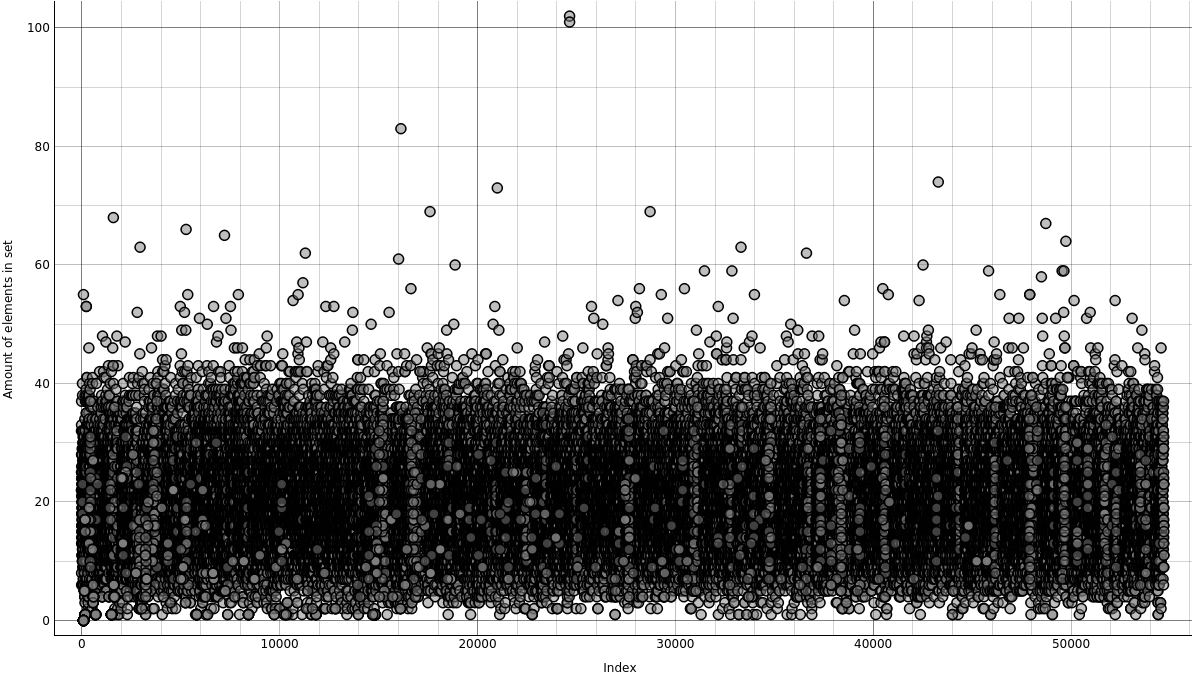
\includegraphics[width=\textwidth]{sets.png}
\caption{\label{fig:sets}Sizes of the sets in Reuters collection.}
\end{figure}

\subsection{Greedy Heuristic by \citeauthor{balas1980set}}
To compare the two extensions, the greedy heuristic was implemented first. As a fast approach to gain a feasible greedy solution to the set cover problem, a procedure by \citeauthor{balas1980set} was used. The running time was quite constant at a value of 202-204 seconds and 19443 sets got into solution. A summary of the results can be found in Table 4.  

\begin{table}[!b]
    \centering
    \begin{tabular}{0.65\textwidth}
      \hline
       & Coverage Rate & Amount of sets in solution &  Best running time in seconds \\
      \hline 
      Value  & 1.0 & 19443  & 202.413  \\
      \hline
    \end{tabular}
    \caption{Results of \textbf{Greedy Heuristic} by  \citeauthor{balas1980set}}
    \label{tab:my_label}
\end{table}




\pagebreak



\subsection{Disk-Friendly Greedy}
As the DFG only needs the sets universe and a p-value to create a solution, a interval from 1.005 to 2.000 was tested on the p-value. 

\citeauthor{Cormode} proposed to limit the size of sub-collections created to a value of 250 sets for each sub-collection $\Sa^{(k)}$. That actually makes the DFG algorithm extremely fast, but as shown in Figure 1, most set sizes are in the same low range of ~40 elements per set. With this limitation, the running time did not pass 60 seconds, but the coverage rate also was lower than .40, which is not satisfying. 

Taking higher sizes, e.g. $|\Sa^{(k)} | = 3000$ raises both the coverage rate and the solution size. The solution with the highest coverage rate in this case made it to a value of .86 at $p= 1.075$, but with a large amount of sets in solution: 33793 sets. That corresponds to nearly 62\% of the whole data set. Whereas the time elapsed for this run was with 139.4 seconds much faster than the greedy algorithm. Figure 2 and 3 present a summary of these tests. 

Without any sub-collection limit, the DFG needed almost the same time as the standard greedy heuristic with about 200-250 seconds. The coverage rate then went up to .90-.99. On closer inspection, it became apparent, that these high coverage rates were only reached by the algorithm adding nearly all sets to solution. For reaching a 0.9 rate, there were added over 40,000 sets; for passing the 0.95 mark it needed 45,000 sets and for beating 0.99 over 52,000.



\subsection{Simulated-Annealing}
At implementation of the simulated annealing it turned out to be a challenge to find a elegant way of checking at each creation of a new solution, if this solution re-covers all un-covered elements that got uncovered by removing sets randomly. It was no expedient solution to check all sets in the whole solution and withdraw all covered elements. In the end it was decided to save all mentions of a element in a hash-array, which was carried on and updated at each solution-finding step. As this updating procedure has to be done twice (at removing sets from solution and bringing other sets into again), this lets the running time shoot upwards. 

The procedure as in \citeauthor{Jacobs1995}, to put set sizes and amount of re-covered elements in relation by introducing a additional parameter for search depth, was not tested out. The reason for disregarding this parameter was, that the computation took to long with the solution not being noticeable shorter. 
As a result it should be recorded, that the important thing in this approach is finding a accurate and fast heuristic to get another feasible solution at every iteration of the simulated annealing.

Apart from the running time, the outstanding power of the simulated annealing lies in finding the optimal solution. The algorithm was run three times for 1500 seconds at each test, with the neighbourhood-scale increasing from .1 to .5 from test to test. As starting solution, the solution of the greedy heuristic by \cite{balas1980set} with 19443 sets was used. The best solution found was with only 10419 sets almost half as long as the greedy solution it began with. 

\begin{table}[!b]
    \centering
    \begin{tabular}{r  c  l}
        Amount of sets & Neighbourhood-Scale & Time elapsed in sec\\
        \hline
        15715 & 0.1 & 1530.449 \\
        11572 & 0.2 & 1798.165 \\
        10727 & 0.3 & 1973.523 \\
        10640 & 0.4 & 2109.728 \\
        10419 & 0.5 & 2000.038 \\
        \hline
        19443 & initial value by Greedy Heuristic 
    \end{tabular}
    \caption{Results of the \textbf{Simulated Annealing}}
\end{table}



\begin{figure}
\centering
\begin{subfigure}[b]{\textwidth}
   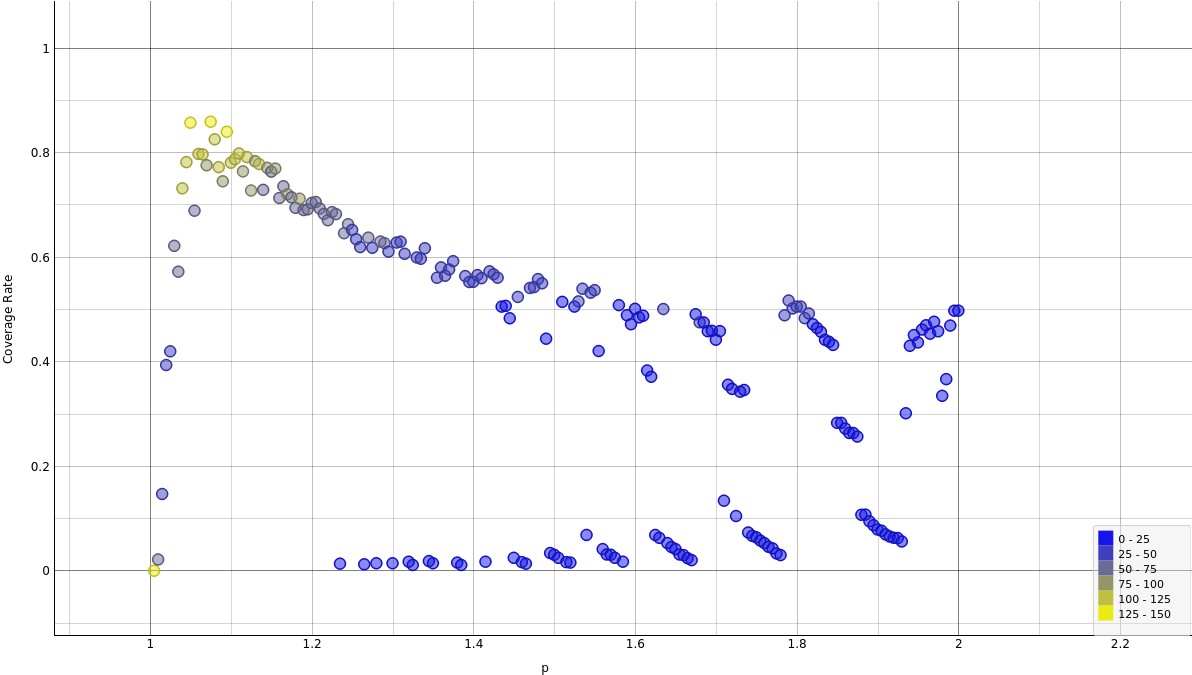
\includegraphics[width=1\linewidth]{dfg_p_crate_time.png}
   \caption{p-Value plotted against coverage rate, colored by the time elapsed in seconds.}
\end{subfigure}

\begin{subfigure}[b]{\textwidth}
   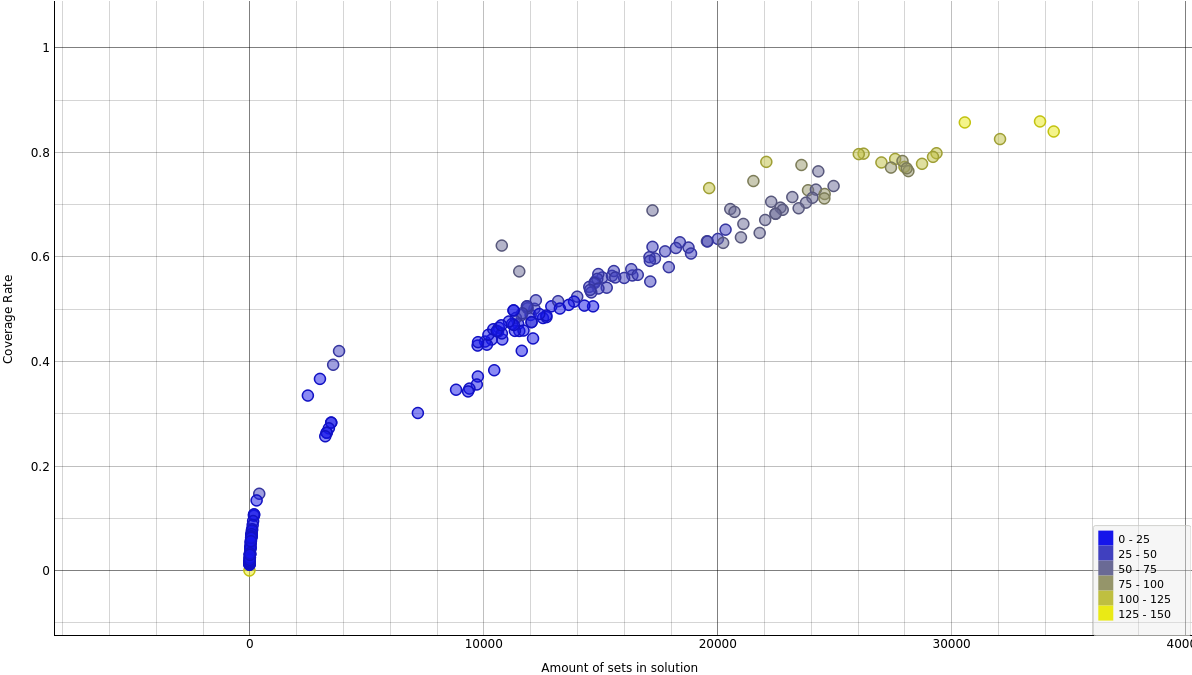
\includegraphics[width=1\linewidth]{dfg_amountsets_crate_time.png}
    \caption{ Amount of sets in solution plotted against coverage rate, colored by the time elapsed in seconds.}
\end{subfigure}
\caption{Results of the \textbf{DFG}-Algorithm}
\end{figure}

\pagebreak

\section{Conclusion}
In this work several ways of solving the Set Cover Problem were tested. The aim was to improve the often used greedy heuristic, which has become kind of a standard procedure for solving this problem. Different aspects were put in the foreground: computation time, coverage rate and size of the solution, that the various approaches lead to. It became apparent, why the strategy of a greedy algorithm is so convincing: with little effort for implementing a greedy heuristic you can get good feasible solutions in quite short time. 

Nevertheless, it can make sense to adapt the greedy heuristic for one's specific application. While only testing the Disk-Friendly-Greeedy by \citeauthor{Cormode} on one data set, which has quite small sets, it can well make sense to use it for very large data sets as mentioned in the paper. Finding a fitting limitation of sub-collection size might give a good trade-off between running time and solution size, which could beat the standard greedy in running time by lengths and save a lot of disk memory. Another point in favour of this algorithm is, that it does not need a universe of elements as reference. Without comparing the solution space with the given element universe, the algorithm manages to find a solution. In a real world example, in which the element universe is not known yet, the DFG can solve this problem extremely fast. 

Putting the optimal solution to the problem in the spotlight, the simulated annealing definitively is a well-performing tool, which will find better solutions to end up with. The challenge is to find a valid neighbouring solution at every step within a reasonable time. Good indexing approaches could solve the running time problem in this particular procedure. If you have enough resources and the quality of the solution needs to be best, simulated annealing is a good way to reach this aim.



\bibliographystyle{IEEEtranN}
%\bibliography{mendeley_v2}
\bibliography{references}
\end{document}